\documentclass[12pt]{report}
\usepackage[a4paper]{geometry}
\usepackage[myheadings]{fullpage}
\usepackage{fancyhdr}
\usepackage{lastpage}
\usepackage{graphicx, wrapfig, subcaption, setspace, booktabs}
\usepackage[T1]{fontenc}
\usepackage[font=small, labelfont=bf]{caption}
\usepackage{fourier}
\usepackage[utf8]{inputenc}
\usepackage[protrusion=true, expansion=true]{microtype}
\usepackage[french]{babel}
\usepackage{sectsty}
\usepackage{url, lipsum}
\newcommand{\HRule}[1]{\rule{\linewidth}{#1}}
\renewcommand{\thesection}{\arabic{section}}
\onehalfspacing
\setcounter{tocdepth}{5}
\setcounter{secnumdepth}{5}

%-------------------------------------------------------------------------------
% HEADER & FOOTER
%-------------------------------------------------------------------------------
\pagestyle{fancy}
\fancyhf{}
\setlength\headheight{15pt}
\fancyhead[L]{FSSM}
\fancyhead[R]{UCA}
\fancyfoot[R]{Page \thepage\ of \pageref{LastPage}}
%-------------------------------------------------------------------------------
% TITLE PAGE
%-------------------------------------------------------------------------------

\begin{document}

\title{ \normalsize \textsc{Université Cadi Ayad,Faculté de              science Smlalia.
        Department Informatique
        Rapport du Projet de XML}
        \\ [2.0cm]
        \HRule{0.5pt} \\
        \LARGE \textbf{\uppercase{Indexation d'un fichier XML}}
        \HRule{2pt} \\ [0.5cm]
        \normalsize \today \vspace*{5\baselineskip}}

\date{}

\author{
        Amri Habiba  \\ 
        Sabri Zineb \\
        Module:Traitement de Document Electronique }

\maketitle
\tableofcontents
\newpage

%-------------------------------------------------------------------------------
% Section title formatting
\sectionfont{\scshape}
%-------------------------------------------------------------------------------

%-------------------------------------------------------------------------------
% BODY
%-------------------------------------------------------------------------------


\newpage
\section{Introduction}
\begin{frame}
\\
\\
Dans le cadre de notre formation de Master Spécialisé en Ingénierie des systèmes d’informations, le module : Traitement de documents nous avons été menés à effectuer un projet, Il s'agit de réaliser un indexateur de document XML.

L’indexation automatique de documents est un domaine de l'informatique et des Sciences de l'information et des bibliothèques qui utilise des méthodes logicielles pour organiser un ensemble de documents et faciliter ultérieurement la recherche de contenu dans cette collection. La multiplicité des types de documents (textuels, audiovisuels, Web) donne lieu à des approches très différentes, notamment en termes de représentation des données. Elles reposent néanmoins sur un socle de théories communes, telles que l'extraction de caractéristiques, le partionnement de données (ou clustering), la quantification, et plus généralement la recherche d'information.

En revanche, les fichiers séquentiels indexés constituent une technique d'usage très général en informatique, pour le stockage de données numériques.

Un index est, en toute généralité, une liste de descripteurs à chacun desquels est associée une liste des documents et/ou parties de documents auxquels ce descripteur renvoie. Ce renvoi peut être pondéré. Lors de la recherche d'information d'un usager, le système rapprochera la demande de l'index pour établir une liste de réponses. En amont, les méthodes utilisées pour constituer automatiquement un index pour un ensemble de documents varient considérablement avec la nature des contenus documentaires à indexer.

Mis à part le développement proprement dit de notre projet, la première étape consistait à saisir le projet puis nous familiariser avec les outils de travail : Lucene et Swing….
\end{frame}\\
\\
\newpage

\section{Qu'est-ce que l'indexation }
L'indexation est une opération humaine de traitement intellectuel d’un document consistant à donner une représentation, par les éléments d’un langage documentaire, des notions résultant de l’analyse d’un document ou d’une question en vue d’en faciliter la recherche [1].
La notion d’indexation documentaire désigne les différents modes d’indexation, pratiqués généralement par les professionnels des bibliothèques et de la documentation, et reposant sur des langages documentaires [2] ou des outils spécifiques (ontologies par exemple). Il s’agit d’une indexation à la fois humaine, manuelle (se distinguant donc de l’indexation automatisée) et contrôlée par des langages documentaires (se distinguant donc de l’indexation libre, notamment des nouvelles formes d’indexation collective).
\section{A quoi cela sert-il}
L'indexation est utilisée pour faciliter la recherche, la classification et l'organisation des objets documentaires. Il est la pierre angulaire de nombreux processus de gestion des connaissances :
Lors d'une recherche documentaire à travers un moteur qui indexe une base de documents : Tous les documents indexés par les mêmes mots clés du langage documentaire sont retrouvés, indépendamment de la langue ou de la présence ou non des mots dans le reste du document.
Lors de l'analyse de corpus (Text Mining) : Les mots clés   sont utilisés pour analyser un corpus textuel avec des méthodes statistiques ou linguistiques et permettent d'obtenir des résultats plus précis.
Pour la veille informationnelle : La sélection de mots clés permet de construire des équations de recherche pour surveiller les sources.
En Linked Open Data : en alignant les différents vocabulaires avec les technologies du web sémantique on peut comparer les termes communs ou différents et enrichir des vocabulaires avec des informations contenues dans les autres vocabulaires (termes équivalents, traduction dans d'autres langues).   Quand   on traite des ensembles de données indexées avec des vocabulaires contrôlés il est plus facile de rechercher de l’information et de lier des données   en utilisant ces vocabulaires. \\
\\
\newpage
\section{Motivation}
\begin{frame}

\\
L'indexation de données essaye de répondre à la question suivante : Comment organiser au mieux une collection de documents afin de pouvoir plus tard retrouver facilement celui qui m'intéresse ?

Une réponse classique consiste à annoter manuellement chaque document d'une série de métadonnées (titre, catégorie(s), date de parution, auteur etc.). Cette approche a l'avantage d'être facile à mettre en œuvre, et de fournir des renseignements de qualité (selon l'expertise de la personne chargée de l'annotation). Cependant, cette solution est ambiguë (un même document pouvant se décrire de plusieurs façons ; on pensera par exemple à l'ambiguïté entre genres musicaux), elle est coûteuse (puisqu'il faut payer un annotateur pour qu'il prenne en charge tout nouveau document dans notre collection), et ne permet de répondre qu'à des requêtes textuelles (à l'inverse d'une requête par image similaire, par exemple).

Face au problème du déluge de données et de l'hétérogénéité croissante des documents que doivent traiter les moteurs de recherche, l'indexation automatique est une nécessité. Elle se base directement sur le contenu, dans le but d'obtenir des résultats univoques et cohérents. En représentant les documents sous forme de vecteurs de descripteurs, il devient possible de les comparer, de mesurer leurs distances les uns des autres, et de répondre à des requêtes de différentes natures.

Les descripteurs de données sont très dépendants du type de média, de même que les algorithmes de recherche par similarité. La prochaine section présente les différentes approches d'indexation en fonction du type des documents à indexer.
\end{frame}
\newpage
\section{MOTEUR D’INDEXATION-RECHERCHE}
Il existe des moteurs d’indexation-recherche uniquement consacrés aux pages web ; ils ne nous intéressent pas beaucoup en termes d’architecture. 
Il existe aussi des moteurs d’indexation-recherche plus génériques, qui peuvent indexer n’importe quoi.\\
Voici une liste des  moteurs plus utilisés:\\
\textbf{Apache Solr} : Serveur de recherche basé sur Lucene.\\
\textbf{Apache Nutch} : Robot d'indexation.\\
\textbf{Apache Hadoop}: Système de fichiers distribué (HDFS) et calcul distribué à l'aide du paradigme MapReduce.\\
\textbf{Apache Tika} : Bibliothèque d'extraction de données et de meta-données pour une très grande variété de formats de fichiers.\\
Le plus célèbre, et sans doutes le plus puissant, est le moteur \textbf{Lucene}, de la fondation Apache, qui a été adopté par pratiquement tous les produits de gestion de contenus et de gestion de documents, qu’ils soient open source ou non. 
Ce qui nous intéresse ici, c’est l’utilisation d’un moteur tel que Lucene dans la gestion des données d'un fichier xml. Un tel moteur a de nombreux atouts :
\begin{enumerate}
\item
Il est plus performant qu’un SGBD sur certaines typologies de requêtes complexes 
\item
Il excelle dans des requêtes qui réunissent contenus structurés et contenus non-structurés. Par « contenus non-structurés », on entend les textes et documents.
\item
Il supporte de très gros volumes sans dégradation des performances. Typiquement plusieurs dizaines de millions d’items sont monnaie courante.
\item
Sa fonction n’est pas de stocker, ni de gérer l’information, il donne juste un moyen de la retrouver par la recherche.

\end{enumerate}
\newpage
\section{Outils}
Lucene appartient au fameux projet Jakarta de la fondation Apache, bien connu pour ses outils tels que Struts ou Tomcat. Cette API écrite en Java se destine à la création de puissants moteurs de recherche orientés texte. Parmi les nombreuses qualités de cette bibliothèque, nous retiendrons essentiellement sa rapidité d'exécution et sa simplicité d'utilisation, tant pour le programmeur que pour l'utilisateur final. La découverte de Lucene se déroulera en deux temps. En premier lieu, nous apprendrons à créer un index à partir de nos documents, pour ensuite soumettre des requêtes au moteur. 
\subsection{Création de l'index}
Toutes les requêtes de recherche effectuées par Lucene s'effectuent sur un index. Il s'agit d'une compilation de mots-clés et de propriétés identifiant des documents. Par exemple, nous pourrons indexer une page HTML grâce aux mots-clés	contenus dans une balise <meta> et conserver en tant que propriétés son URL complète et son titre. 
Lors de la création d'un index, la bibliothèque crée un nouveau répertoire contenant plusieurs fichiers appelés des segments. Vous pourrez vous reporter au site officiel de Lucene (http://jakarta.apache.org/lucene) pour obtenir des informations sur la structure de ces fichiers. 
Les classes nécessaires à la création d'un nouvel index, ou à l'extension d'un existant, se trouvent dans les paquetages org.apache.lucene.index et org.apache.lucene.analysis.standard. Le premier contient l'outil de création de l'index tandis que le second accueille les analyseurs de texte. En effet, pendant la création de l'index, Lucene fait appel à des tokenizers et des filtres. Ceux-ci permettent respectivement de découper le texte et de lui appliquer des modifications. Ainsi, le StandardAnalyser découpe le texte mot par mot, les met en minuscules puis retire ceux qui sont inutiles (comme en anglais "the" ou "and"). Vous pouvez bien entendu créer vos propres combinaisons de filtres, et même en créer de nouveaux. 
Une fois un analyseur créé, nous pouvons construire une instance d'IndexWriter et lui ajouter des documents. Le listing 1 expose la manière de la créer. 
Le premier paramètre du constructeur d'IndexWriter désigne le nom du répertoire dans lequel sera enregistré l'index. Le dernier paramètre permet pour sa part de contrôler le mode de création de l'index. Lorsqu'il vaut true, un nouvel index sera créé, au risque de supprimer celui existant. En choisissant la valeur false, nous demandons à Lucene d'ajouter les informations du nouvel index à celui existant. 
Une fois l'IndexWriter créé, il incombe au programmeur de compiler des documents par l'intermédiaire de la classe Document du paquetage org.apache.lucene.document, et de les placer dans l'index. Notre programme réalise cette tâche dans la méthode addDocument (). Un document se compose lui-même de champs, concrétisés par des instances de la classe Field. Le listing 2 présente l'ajout de champs à un document, puis l'ajout dudit document à l'index. Ce code source expose les trois sortes de champs que nous pouvons placer dans un document : non indexé, non stocké et stocké/indexé. 
Le type non indexé, que nous pouvons réaliser par l'intermédiaire de la méthode utilitaire UnIndexed (), sert à ajouter des caractéristiques à un document, lesquelles ne seront pas affectées par l'analyseur. Dans notre exemple, nous ajoutons l'URL de cette manière afin de la présenter lors des résultats de recherche. Le deuxième type se voit affecté par l'analyseur, mais nous pouvons par la suite récupérer la valeur employée pour créer le champ. Enfin, nous avons à notre disposition le type Text(), qui est en même temps indexé et accessible. 
La méthode addDocument() de WebIndex pousse le concept un peu plus loin en indexant toutes les pages HTML liées depuis celle choisie par l'utilisateur. Ce travail repose sur la classe interne HTTPDocument qui fait un usage intensif des expressions régulières.
\subsubsection{Formats de fichier index}
Un index contient une séquence de documents.
\begin{itemize}
\item
Un document est une séquence de champs
\item
Un champ est une séquence nommée de termes
\item
Un terme est une chaîne
\end{itemize}
\subsubsection{Segments}
Les indices de Lucene peuvent être composés de plusieurs sous-indices ou segments . Chaque segment est un index entièrement indépendant, qui pourrait être recherché séparément. Les indices évoluent en:
\begin{enumerate}
\item
Création de nouveaux segments pour les nouveaux documents ajoutés.
\item
Fusion des segments existants.
\end{enumerate}
Les recherches peuvent impliquer plusieurs segments et / ou plusieurs index, chaque index étant potentiellement composé d'un ensemble de segments.


\subsubsection{Résumé des extensions de fichier}
\newpage
\begin{flushleft}
\begin{table}
\caption{Le tableau suivant résume les noms et les extensions des fichiers dans Lucene:}
\begin{tabular}{|c|c|c|}
\hline
NOM & EXTENTION & Brève Description\\
\hline\hline
Fichier Segments & .gen &segments N Stocke des informations sur les segments\\
Fichier de verrouillage	& Write.lock	& Le verrouillage d'écriture empêche plusieurs indexeurs d'écrire sur le même fichier.\\
Fichier composé	& .cfs	&  Un fichier «virtuel» facultatif composé de tous les autres fichiers d'index .\\
Des champs	& .fnm	& Stocke des informations sur les champs\\
Index des champs	& .fdx	& Contient des pointeurs vers les données de champ\\
Données sur le terrain	 &.fdt	& Les champs stockés pour les documents\\
Informations générales	& .tis &	 Partie du dictionnaire de termes, stocke l'information de terme\\
Term Info Index	& .tii &	 L'index dans le fichier Term Infos\\
Fréquences	& .frq	& Contient la liste des documents contenant chaque terme avec la fréquence\\
Positions	& .prx	& Stocke les informations de position sur l'endroit où un terme se produit dans l'index\\
Normes	& .nrm	& Encode les facteurs de longueur et d'amplification des docs et des champs\\
Terme vecteur Index	 & .tvx	& Stocke le décalage dans le fichier de données du document\\
Documents vectoriels à terme	& .tvd	& Contient des informations sur chaque document qui comporte des vecteurs à terme\\
Champs de vecteurs temporaires	&  .tvf	& L'information au niveau du terrain sur les vecteurs à terme\\
Documents supprimés	 & .del	& Informations sur les fichiers supprimés\\
\hline\end{tabular}
\label{table:precision}
\end{table}
\end{flushleft}
\subsection{Lucene Classes d'indexation}

	\begin{frame}
\newline
	 la liste des classes couramment utilisés au cours du processus d'indexation\newline
	 
		\textbf{IndexWriter:}
		\newline
Cette classe agit comme un élément de base qui crée mises à jour des index pendant le processus d'indexation.
		\newline
		
		\textbf{Annuaire:}\newline
Cette classe représente l'emplacement de stockage des index.
\newline

\textbf{Analyzer:}\newline
Classe Analyzer est responsable d'analyser un document et obtenir les jetons / mots du texte qui doit être indexé. Sans l'analyse faite, IndexWriter ne peut pas créer un index.
\newline
\newpage
\textbf{Document:}\newline
Document représente un document virtuel avec les champs où le terrain est objet qui peut contenir le contenu du document physique, ses méta données et ainsi de suite. Analyzer peut comprendre un document uniquement.
\newline

\textbf{Champ:}\newline
 Le champ est l'unité la plus basse ou le point du processus d'indexation de départ. Il représente la clé relation où une clé est utilisée pour identifier la valeur à indexer la valeur paire. Dites un champ utilisé pour représenter le contenu d'un document aura clé comme «contenu» et la valeur peut contenir la totalité ou une partie du texte ou du contenu numérique du document.	

      
		\end{frame}
\subsection{Lucene Opérations d'indexation}

\begin{frame}
\newline
\textbf{la liste des opérations couramment utilisés au cours du processus d'indexation}\newline
\begin{itemize}
\item \textbf{Ajouter un document:}Cette opération est utilisée dans l'étape initiale du procesus d'indexation pour créer l'index du contenu nouvellement disponibles.
\item \textbf{Mise à jour du document:}Cette opération est utilisée pour mettre à jour les index pour refléter les changements dans le contenu mis à jour. Il est semblable à recréer l'index.
\item \textbf{Supprimer le document:}Cette opération est utilisée pour mettre à jour les index pour exclure les documents qui ne sont pas tenus d'être indexés / recherché.
\item \textbf{Options Champ:}options de champ indique une manière ou contrôle la façon dont le contenu d'un champ sont à effectuer des recherches.
\end{itemize}
\end{frame}
\newpage
\subsection{Lucene Processus d'indexation}
processus d'indexation est l'une des fonctionnalités de base fournies par Lucene. Le diagramme suivant illustre le processus d'indexation et l'utilisation des classes. IndexWriter est le composant le plus important et le noyau du processus d'indexation.
\newline\newline
 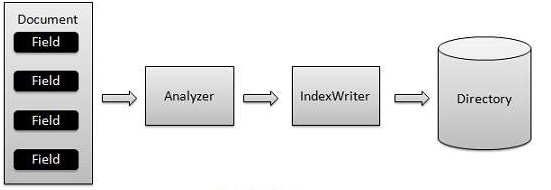
\includegraphics[height=\dimexpr4\textheight/16\relax]{2}
  % \caption{processus d'indexation}


\section{Effectuer une recherche}
Les classes relatives aux recherches se situent dans les paquetages org.apache.lucene.search et org.apache.lucene.queryParser.

\subsection{Lucene Recherche opération}
le processus de recherche est l'une des fonctionnalités de base fournies par Lucene. Le diagramme suivant illustre le processus de recherche et l'utilisation des classes. IndexSearcher est le composant le plus important et le noyau du processus de recherche.
\newline\newline\newline
  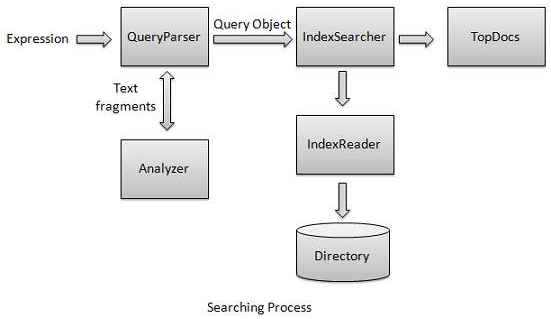
\includegraphics[height=\dimexpr6\textheight/16\relax]{1}
    
 
\section{Requêtes}
\begin{frame}


A partir d'un index, notre application peut permettre à l'utilisateur de saisir des requêtes pour lui retourner les résultats pertinents. La syntaxe acceptée par Lucene pour les requêtes se révèle particulièrement puissante, bien que relativement simple. Outre les traditionnels modificateurs "+" et "-", les jokers "*" et « ? » ainsi que les opérateurs booléens "AND", "OR" et "NOT" (que nous pouvons raccourcir en "\&\&", « || » et « ! »), nous avons accès à deux fonctionnalités particulièrement intéressantes. Ainsi, l'accent circonflexe, placé à la fin d'un mot, permet d'augmenter la priorité d'un mot. Ainsi, dans la requête "cpp OR java\^", Lucene choisira en priorité le terme "java". Cet opérateur peut être suivi d'un chiffre positif définissant la valeur de la priorité. A cela s'ajoute l'opérateur tilde "\~" qui trouve un emploi dans deux situations. Dans l'exemple "java lucene"\~5, le moteur cherchera les termes java et Lucene situés à une distance de moins de 5 mots l'un de l'autre. Par contre, la recherche de "form~" renverra tous les mots similaires à "form", ce qui inclut par exemple "farm" ou "firm". Enfin, nous pouvons effectuer des requêtes sur des champs particuliers des documents en préfixant les requêtes par le nom du champ suivi du caractère deux-points, comme dans "titre : Lucene".
\end{frame}

\section{Conclusion et perspectives}

Dans ce projet, nous avons proposé une approche pour l’indexation et la recherche dans les documents XML sachant qu’on était intéressée à deux problèmes de fouille de textes : l’extraction automatique de termes-clés dans des documents XML et la classification.
Parmi les perspectives, nous envisageons d’intégrer d’autres descripteurs de formes pour enrichir notre système. Tester d’autres techniques d’indexation pour le problème d’extraction automatique de termes-clés on peut même définir une nouvelle mesure, le DPM-index, qui discrimine les phrases (n-grammes) qui se chevauchent dans un document. Pour le problème de classification dans des catégories prédéfinies, on envisage à combiner les métriques afin d’arriver à faire la classification et sa qualité.

%-------------------------------------------------------------------------------
% REFERENCES
%-------------------------------------------------------------------------------
\newpage

\bibliographystyle{abbrv}
%\bibliography{sigproc}

\begin{thebibliography}{1}

\bibitem{rankAggregation}
https://fr.wikipedia.org/wiki/Lucene
\bibitem{rankAggregation}
http://www.lucenetutorial.com/
\bibitem{bundleReco}
http://lucene.apache.org/
\bibitem{bundleReco}
http://www.torrefacteurjava.fr/content/
\bibitem{bundleReco}
https://wiki.apache.org/lucene-java/
\bibitem{bundleReco}
http://www.w3ii.com/fr/lucene/default.html
\bibitem{bundleReco}
https://wiki.apache.org/lucene-java/
\bibitem{bundleReco}
http://www.w3ii.com/fr/lucene/default.html
\bibitem{bundleReco}
http ://jakarta.apache.org/lucene
\bibitem{bundleReco}
http://blog.soat.fr/2010/09/comment-utiliser-lucene-dans-vos-applications/
\bibitem{bundleReco}
http://www.journaldunet.com/solutions/saas-logiciel/5-moteurs-de-recherche-open-source/apache-lucene.shtml
\bibitem{simrank}
M. McCandless, E. Hatcher, and O. Gospodnetić.
\newblock Livre:  {\em Lucene In Action}
\bibitem{simrank}
Introduction to Apache Lucene: Construction of Java Open Source Full Text Retrieval Systems" by Koshi Sekiguti ; Gijutsu-Hyohron Co.
\bibitem{simrank}
Manfred Hardt, Dr. Fabian Theis: "Suchmaschinen entwickeln mit Apache Lucene"; Software  Support Verlag, Francfort-sur-le-Main, Allemagne; septembre 2004.
\bibitem{simrank}
http://fadben.asso.fr/wikinotions/index.php/
\bibitem{simrank}
http://gfx.developpez.com/tutoriel/java/lucene/
\bibitem{simrank}
http://infrastructure.smile.eu/Tout-savoir-sur/Principes-d-architecture-et-outils-open-source/La-gestion-des-donnees/Le-moteur-d-indexation-recherche
\end{thebibliography}

\end{document}
